\section{Experimental Results}

In order to evaluate our method, we use the BCI Competition IV dataset 2a \citep{brunner2008bci}, which contains 4-class motor imagery EEG data from 9 subjects. Each subject participated in two sessions of 6 runs on different days. The training data is from the first session, and the test data is from the second. A run consist of 48 labeled trials, divided evenly between the 4 classes. Each trial measured the brain signals of a subject on 22 EEG channels and 3 EOG channels. We disregard the EOG channels since we are interested in correcting artifacts without any reference signals. Examples of trials, channels, runs, and sessions are shown in \cref{fig:dataset}. What we refer to as a trial is three second span (750 samples) of motor imagery, i.e., without the cue, break, etc. in between.

\begin{figure*}
	\centering
	\begin{adjustbox}{width=\textwidth}
		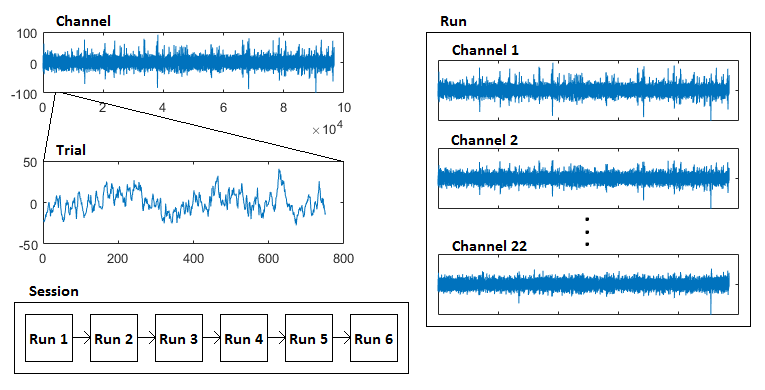
\includegraphics{figures/bciiv2a.png}
	\end{adjustbox}
	\caption{Sessions, runs, channels, trials, and the relations between them.}
	\label{fig:dataset}
\end{figure*}

We set up two pipelines to be compared. The first consists of OACL, followed by FBCSP and Random Forest. The second is without the OACL step, i.e., just FBCSP and Random Forest. We run Random Forest with six predefined seeds and return the mean to ensure reproducibility. We perform 6-fold cross-validation on the training data using five runs for training and one for validation. We ran 200 iterations of Bayesian Optimization of select hyperparameters for each pipeline. The best hyperparameters for each pipeline is then used for the final evaluation where we try to predict the labels for the test data. We repeat this for each subject. \Cref{fig:results} shows the obtained accuracies and KAPPA scores for each subject.

To determine the significance of these results we use the Wilcoxon signed-rank test. \Cref{fig:wilcoxon} shows the results of the test.

\begin{table}[H]
	\centering
	\caption{Wilcoxon signed-rank test}
	\label{fig:wilcoxon}
	\begin{tabular}{@{}l|llll@{}}
		\toprule
		S & No OACL & OACL & Diff & Rank \\ \midrule
		1 &   83,04            &                 &      &      \\
		2 &   57,18            &                 &      &      \\
		3 &   78,18            &                 &      &      \\
		4 &   65,74            &                 &      &      \\
		5 &   58,85            &                 &      &      \\
		6 &   50,23            &                 &      &      \\
		7 &   68,75            &                 &      &      \\
		8 &   74,54            &                 &      &      \\
		9 &   75,64            &                 &      &      \\ \bottomrule
	\end{tabular}
\end{table}

\subsection{Discussion}\label{sec:discussion}
\todo{discuss that optimal filterbank ranges are different from subject to subject}
In the original OACL paper by \citep{li2015ocular}, the relative heights ranges specified in \cref{eq:ranges} were determined by manual inspection of the characteristics of ocular artifacts. Since we generalised this as an optimization of hyperparameter, the found ranges are no longer guaranteed to be optimal in regards to ocular artifacts, but instead optimized for correcting the noise that most negatively affects the classification results. In fact, since we optimize the ranges for maximal classification accuracy, the method may be removing parts of the signal that are technically not artifacts, but removing them increases the performance of the classification model.

Moreover, we have run the Bayesian optimization with the default settings with regards to exploration vs. exploitation. Since running experiments on the pipeline with OACL is quite expensive, it would be better to tune the Bayesian optimization to spend more time on selecting the best candidate future sample to perform the next experiment on.

As explained in \cite{hoffmann2008correction}, residual artifacts were still present after noise reduction methods were applied. We have also observed that residual artifacts are present, this can be seen in \cref{fig:oacl-signals}, where an event is registered around $x \approx 170$, but the following desynchronization/synchronization is not registered. A way that this could be handled was to run a sub-functionality whenever an artifact is registered that checks if a residual artifact is present, and mark it. These signals might need another $\theta$, since these artifacts are quite different from the artifacts introduced by eye blinks.
\todo{skriv at man kunne håndtere residuals evt. ved kald til subroutine in konstruktionen af et artifact signal.}